\documentclass[12pt]{article}

\usepackage{sbc-template}
\usepackage{graphicx,url}
\usepackage[brazil]{babel}
\usepackage[utf8]{inputenc}
\usepackage{float}
\usepackage{geometry}
\usepackage{enumitem}
\usepackage{hyperref}
\usepackage{array}
\usepackage{booktabs}

\sloppy

% ─── PÁGINA 1: Formato Artigo SBC ─────────────────────────────────────────────

\title{WhyRunner: Online Judge Educacional com Feedback por Inteligência Artificial}

\author{Juan Israel dos Anjos\inst{1}}

\address{Instituto Federal de Educação, Ciência e Tecnologia de Minas Gerais (IFMG)\\
  Rua Afonso Sardinha, 90, Ouro Branco/MG, CEP: 36494-018, Brasil
  \email{juaniwk3@gmail.com}
}

\begin{document}

\maketitle

\begin{abstract}
WhyRunner is an educational online judge system designed to support programming
teaching in formal academic environments. The platform integrates secure
containerized code execution, real-time contest management, a professor-curated
Class/Lesson/Exercise assignment model, AI-assisted problem authoring, and
AI-powered pedagogical feedback using Google Gemini. Unlike traditional judges
that return only binary verdicts, WhyRunner provides contextual, student-initiated
hints that guide learning without revealing solutions, and lets professors assemble
gradable lessons from existing problems outside of timed contests. The system is
fully implemented and self-tested by the author; classroom evaluation with real
students and instructors has not yet been conducted and is planned as next step.
The software is open-source (MIT) and targets secondary, technical, and higher
education contexts.
\end{abstract}

\begin{resumo}
O WhyRunner é um sistema de juiz online educacional desenvolvido para apoiar o
ensino de programação em ambientes acadêmicos formais. A plataforma integra
execução segura de código em contêineres, gerenciamento de competições em tempo
real, um modelo de aulas curadas pelo docente (Turma/Aula/Exercício), autoria de
problemas assistida por IA e feedback pedagógico gerado por inteligência
artificial (Google Gemini). Diferentemente dos juízes tradicionais, que retornam
apenas veredictos binários, o WhyRunner fornece dicas contextuais, acionadas pelo
próprio estudante, que orientam o aprendizado sem revelar a solução, além de
permitir que docentes montem aulas avaliáveis a partir de problemas existentes,
fora do contexto de competições cronometradas. O sistema está totalmente
implementado e foi testado pelo próprio autor; a avaliação em sala de aula com
estudantes e docentes reais ainda não foi realizada e é o próximo passo
planejado. O software é de código aberto (MIT) e destina-se aos contextos de
ensino médio, técnico e superior.
\end{resumo}

% ─── PÁGINAS 2–4: White Paper ─────────────────────────────────────────────────

\newgeometry{margin=2cm}

\section*{1. Contexto Educacional}

O ensino de programação e pensamento computacional é previsto na
\textbf{BNCC-Computação} (Resolução CNE/CP nº 2/2022) como eixo estruturante do
currículo de Computação na Educação Básica e permeia a formação técnica e
superior em Ciências Exatas e Engenharias. Entre os objetos de aprendizagem
diretamente atendidos pelo WhyRunner estão:

\begin{itemize}[nosep]
  \item \textbf{Pensamento Computacional}: decomposição de problemas,
        reconhecimento de padrões, algoritmos e depuração de código;
  \item \textbf{Mundo Digital}: desenvolvimento e teste de programas,
        ambientes de execução e boas práticas de engenharia de software;
  \item \textbf{Cultura Digital}: participação em práticas colaborativas e
        competitivas mediadas por tecnologia.
\end{itemize}

No Ensino Médio, o software apoia a competência específica
\textbf{EM13CO105} (desenvolver e implementar programas computacionais para a
solução de problemas) e, no Ensino Técnico/Superior, complementa disciplinas de
Algoritmos, Estruturas de Dados e Programação Competitiva.

A abordagem pedagógica é \textbf{construtivista}: o estudante resolve
problemas de forma autônoma, recebe feedback imediato do juiz automático e,
quando necessário, solicita dicas contextuais geradas por IA, que orientam o
raciocínio sem entregar a resposta.

\section*{2. Objetivo}

O WhyRunner tem como propósito fornecer aos docentes uma ferramenta gratuita,
moderna e de fácil configuração para \textbf{criar e gerenciar competições de
programação em sala de aula}, e aos estudantes uma experiência de submissão com
\textbf{feedback formativo imediato}, sem depender de plataformas comerciais
ou de infraestrutura complexa.

\section*{3. Público-Alvo}

\begin{itemize}[nosep]
  \item \textbf{Ensino Médio Integrado / Técnico}: estudantes de cursos técnicos
        em Informática, Desenvolvimento de Sistemas e áreas afins (a partir do
        1º ano);
  \item \textbf{Graduação}: estudantes de Ciência da Computação, Engenharia de
        Computação, Sistemas de Informação e correlatos (todos os semestres);
  \item \textbf{Docentes}: professores que ministram disciplinas de programação
        e desejam conduzir avaliações práticas automatizadas.
\end{itemize}

Necessidades identificadas: feedback além do ``Wrong Answer''; controle de
tempo real durante provas; histórico de submissões por aluno; interface em
Português.

\section*{4. Diferenciais e Potenciais de Inovação}

\begin{center}
\begin{tabular}{lccccc}
\toprule
\textbf{Funcionalidade} & \textbf{BOCA} & \textbf{Run Codes} & \textbf{Ataux} & \textbf{WhyRunner} \\
\midrule
Feedback por IA            & Não & Não & Não & \textbf{Sim} \\
Interface em Português     & Não & Sim & Sim & \textbf{Sim} \\
Código aberto (MIT)        & Sim & Não & Não & \textbf{Sim} \\
Sem fila externa           & N/A & Não & Não & \textbf{Sim} \\
Scoreboard em tempo real   & Sim & Sim & Não & \textbf{Sim} \\
Aulas curadas pelo docente & Não & Não & Não & \textbf{Sim} \\
Restrição de solução (algoritmo exigido) & Não & Não & Não & \textbf{Sim} \\
\bottomrule
\end{tabular}
\end{center}

\vspace{0.5em}
O principal diferencial é o \textbf{feedback pedagógico via IA}: ao solicitar
ajuda, o estudante recebe uma dica contextual gerada pelo Google Gemini, que
analisa o código enviado, os casos de teste com falha e o enunciado do problema,
retornando uma orientação que estimula o raciocínio sem revelar a solução. A IA
é instruída explicitamente a \emph{não} fornecer o código correto.

Um segundo diferencial é o \textbf{modelo de Turma/Aula/Exercício}: o docente
monta uma aula a partir de problemas existentes, o aluno submete a aula
inteira de uma vez e a nota por exercício é calculada automaticamente pelo
juiz, com feedback em texto livre do docente. Um terceiro diferencial é a
\textbf{restrição de solução}: além de bater a saída esperada, o docente pode
exigir um limite estrutural (ex.: profundidade máxima de laços) ou um
algoritmo específico (ex.: ``deve usar Dijkstra''), este último verificado por
classificação via IA sobre o código. Uma submissão que viola qualquer
restrição não conta para o placar nem para conclusão do problema, mesmo tendo
passado em todos os casos de teste.

\section*{5. Repercussões Educacionais Esperadas}

O WhyRunner ainda não foi implantado em sala de aula com estudantes e
docentes reais; nenhuma avaliação foi conduzida até o momento. Com base no
desenho do sistema, espera-se que:
\begin{itemize}[nosep]
  \item o feedback contextual por IA dê ao estudante mais clareza sobre
        \emph{por que} uma solução falhou, em contraste com o veredicto
        ``Wrong Answer'' puro;
  \item o feedback automático reduza interrupções durante provas dirigidas ao
        docente;
  \item o scoreboard em tempo real aumente o engajamento competitivo;
  \item o processamento assíncrono via \texttt{LISTEN/NOTIFY} mantenha as
        submissões rápidas mesmo sob carga.
\end{itemize}
Essas expectativas serão verificadas na avaliação em sala de aula planejada
como próximo passo (Seção~8).

\section*{6. Aspectos Tecnológicos}

\begin{itemize}[nosep]
  \item \textbf{Frontend / API}: Next.js 16 (App Router, Server Actions), React
        19, TypeScript, Tailwind CSS v4, Monaco Editor;
  \item \textbf{Judge worker}: Rust (Tokio async runtime, sqlx);
  \item \textbf{Banco de dados}: PostgreSQL + Drizzle ORM; comunicação
        inter-serviço via \texttt{LISTEN/NOTIFY} nativo (sem fila externa);
  \item \textbf{Autenticação}: Better Auth (e-mail/senha, GitHub, Google OAuth);
  \item \textbf{Execução de código}: Docker, contêineres efêmeros com
        \texttt{--cpus 0.5 --memory 128m}, sem acesso à rede;
  \item \textbf{IA}: Google Gemini 2.0 Flash (API REST via Server Action):
        dica de feedback, rascunho/revisão de problema, narrativa temática e
        classificação de restrição de algoritmo;
  \item \textbf{Validação pré-publicação}: solução de referência do docente
        executada no sandbox do juiz antes de publicar; edição de I/O
        invalida uma validação aprovada;
  \item \textbf{Restrições de solução}: limites estruturais (análise
        estática) e algoritmo exigido (classificação por IA), aplicados após
        a submissão passar em todos os casos de teste;
  \item \textbf{Linguagens suportadas}: Python, Rust, C++, Portugol (em
        produção); C e Java arquiteturalmente suportados, pendentes de
        implementação no runner;
  \item \textbf{Runtime}: Bun (gerenciador de pacotes e runtime Node.js);
  \item \textbf{Notificações}: caixa de entrada in-app (submissão avaliada,
        pedido/aprovação de entrada em competição, aula desbloqueada), com
        contagem de não lidas e agregação de eventos repetidos do mesmo
        tipo;
  \item \textbf{Licença}: MIT;
  \item \textbf{i18n}: next-intl (Português e Inglês).
\end{itemize}

\subsection*{Arquitetura resumida}

\begin{enumerate}[nosep]
  \item Usuário submete código pelo editor web (Monaco), seja em uma
        competição ou em um exercício de aula;
  \item Server Action valida, salva \texttt{PENDING} no PostgreSQL e emite
        \texttt{NOTIFY};
  \item Judge worker (Rust) recebe notificação, executa código em Docker,
        compara saídas com gabarito; para exercícios de aula, todos os
        casos de teste são executados (não apenas até a primeira falha),
        para computar a nota do exercício como fração de casos aprovados;
  \item Se o problema tiver restrições de solução, o worker roda análise
        estática e/ou classificação por IA antes de finalizar o resultado;
  \item Resultado (\texttt{PASSED / FAILED / TLE / ERROR} ou violação de
        restrição) é gravado no banco;
  \item Frontend atualiza em tempo real via TanStack Query e gera uma
        notificação in-app para o usuário;
  \item Em falha, estudante pode solicitar dica da IA (Gemini).
\end{enumerate}

\subsection*{Modelo Turma/Aula/Exercício}

\begin{enumerate}[nosep]
  \item Docente cria uma turma (\texttt{classroom}) com código de entrada;
  \item Docente monta uma aula (\texttt{lesson}) adicionando problemas
        existentes como exercícios (\texttt{exercise}) ordenados, com prazo
        opcional, e publica para a turma;
  \item Aluno entra na turma pelo código, responde cada exercício e submete
        a aula inteira de uma vez (\texttt{lessonSubmission});
  \item Após o prazo, docente revisa: nota por exercício calculada
        automaticamente pelo juiz e feedback em texto livre por exercício.
\end{enumerate}

\section*{7. Apresentação do Software}

\begin{figure}[H]
\centering
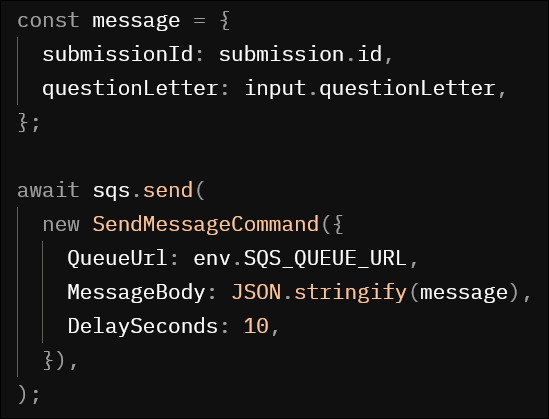
\includegraphics[width=0.85\textwidth]{send.png}
\caption{Tela de submissão de código com editor Monaco integrado.}
\end{figure}

\begin{figure}[H]
\centering
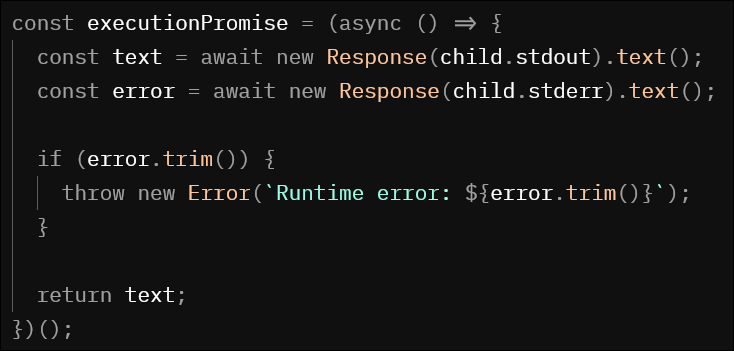
\includegraphics[width=0.85\textwidth]{result.png}
\caption{Tela de resultado: casos de teste, status por caso e opção de solicitar feedback por IA.}
\end{figure}

\section*{8. Considerações Finais}

O WhyRunner demonstra que é possível combinar execução segura de código,
gerenciamento de contest, um modelo de Turma/Aula/Exercício curado pelo
docente, autoria de problemas assistida por IA (rascunho, revisão e
narrativa), restrições de solução e feedback pedagógico por IA em uma única
plataforma gratuita e de código aberto. O sistema está funcionalmente
completo e pronto para implantação por docentes, sem necessidade de
infraestrutura proprietária, mas ainda não foi avaliado com estudantes e
docentes reais; essa avaliação é o próximo passo. A arquitetura é extensível
para suportar novos idiomas de programação, detecção de plágio e avaliação
quantitativa de usabilidade.

\subsection*{Nível TRL}

\textbf{TRL 4--5: Validação/demonstração de tecnologia em ambiente relevante}:
O WhyRunner está implementado e foi testado pelo próprio autor, mas ainda não
foi implantado ou operado com um público real de estudantes e docentes. Uma
implantação em ambiente operacional (sala de aula real) é necessária para
avançar a TRL 6--7.

\bibliographystyle{sbc}
\bibliography{refs}

\end{document}
